\documentclass[10pt,twocolumn,letterpaper]{article}

% ---------- Fonts & Encoding ----------
\usepackage[utf8]{inputenc}
\usepackage[T1]{fontenc}
\usepackage{libertine}
\usepackage[libertine]{newtxmath}
\usepackage[scaled=0.85]{beramono}

% ---------- Page Layout ----------
\usepackage[margin=0.85in,columnsep=0.3in]{geometry}
\usepackage{parskip}
\setlength{\parskip}{4pt plus 1pt minus 1pt}

% ---------- Section Formatting ----------
\usepackage{titlesec}
\titleformat{\section}{\large\bfseries\sffamily}{\thesection}{0.8em}{}
\titleformat{\subsection}{\normalsize\bfseries\sffamily}{\thesubsection}{0.7em}{}
\titlespacing*{\section}{0pt}{14pt plus 2pt}{6pt plus 1pt}
\titlespacing*{\subsection}{0pt}{10pt plus 2pt}{4pt plus 1pt}

% ---------- Math & Theorems ----------
\usepackage{amsmath}
\let\Bbbk\relax
\usepackage{amssymb}
\let\openbox\relax
\usepackage{amsthm}
\newtheorem{theorem}{Theorem}
\newtheorem{definition}{Definition}
\newtheorem{corollary}{Corollary}
\newtheorem{lemma}{Lemma}

% ---------- Tables ----------
\usepackage{booktabs}
\usepackage{tabularx}
\renewcommand{\arraystretch}{1.15}

% ---------- Figures & Graphics ----------
\usepackage{graphicx}
\usepackage{tikz}
\usetikzlibrary{positioning,arrows.meta,shapes.geometric,fit,backgrounds,calc}
\usepackage{caption}
\captionsetup{font=small,labelfont=bf,skip=6pt}

% ---------- Code Listings ----------
\usepackage{listings}
\usepackage{xcolor}
\definecolor{codebg}{HTML}{F7F7F8}
\definecolor{codeframe}{HTML}{E0E0E0}
\definecolor{kw}{HTML}{1A5276}
\definecolor{cmt}{HTML}{6C7A89}
\lstdefinestyle{code}{
    basicstyle=\ttfamily\footnotesize,
    breaklines=true,
    frame=single,
    framesep=6pt,
    xleftmargin=6pt,
    xrightmargin=2pt,
    backgroundcolor=\color{codebg},
    rulecolor=\color{codeframe},
    keywordstyle=\color{kw}\bfseries,
    commentstyle=\color{cmt}\itshape,
    numbers=none,
    captionpos=b,
    aboveskip=8pt,
    belowskip=8pt,
}
\lstset{style=code}

% ---------- Hyperlinks ----------
\usepackage[colorlinks=true,linkcolor=blue!50!black,citecolor=blue!50!black,urlcolor=blue!50!black]{hyperref}
\usepackage{url}
\usepackage{enumitem}

% ---------- Header ----------
\usepackage{fancyhdr}
\pagestyle{fancy}
\fancyhf{}
\renewcommand{\headrulewidth}{0.4pt}
\fancyhead[L]{\small\sffamily Private Decentralized Inference on Apple Silicon}
\fancyhead[R]{\small\sffamily\thepage}
\fancyfoot{}

% =====================================================================
\title{%
\vspace{-0.5cm}
{\LARGE\sffamily\bfseries Private Decentralized Inference\\on Apple Silicon}\\[8pt]
{\large\sffamily Eliminating Software Access Paths Without Hardware TEEs}
}

\author{
    \textbf{Gajesh Naik} \\[4pt]
    {\small Eigen Labs} \\[2pt]
    {\small\texttt{gajesh@eigenlabs.org}}
}

\date{\small March 2026}

% =====================================================================
\begin{document}

\twocolumn[
\maketitle
\thispagestyle{fancy}

% ---------- Abstract ----------
\begin{@twocolumnfalse}
\begin{abstract}
\noindent
When you use a cloud AI service, your prompts travel to someone else's server. You trust them not to read, store, or misuse your data---but that trust is based on a privacy policy, not a technical guarantee.

DGInf changes this. It is a platform where Mac owners rent out their idle compute for AI inference, and consumers get privacy they can verify---not just trust. The consumer's prompts are processed on the provider's Mac, but the provider cannot see them.

The challenge is that Apple Silicon Macs have no hardware ``secure vault'' (called a TEE) that can lock away data during computation. The Secure Enclave---Apple's security chip---can generate keys and sign things, but it cannot encrypt the Mac's main memory or hide what the GPU is computing.

We solve this the same way Apple does for its own Private Cloud Compute service: instead of encrypting memory, we \emph{remove every software tool that could be used to look at it}. Debuggers are blocked at the kernel level. Memory-reading APIs are denied. The operating system's integrity protections cannot be disabled without rebooting---which erases all data. An independent Apple MDM server verifies the Mac's security settings directly, catching any provider who tries to weaken their system.

The result: the only way to extract inference data is to physically probe the memory chips---which are soldered into the processor and require lab equipment to access. This is the same level of protection Apple provides for Siri and Apple Intelligence queries in its own data centers.

We also show that this approach is economically viable. Modern AI models with Mixture-of-Experts architectures are 6 to 32 times cheaper to run on a Mac than through cloud providers, creating a marketplace where consumers save money and Mac owners earn passive income from hardware they already own.

The system is validated end-to-end on real Apple Silicon hardware with live inference and hardware-verified trust.
\end{abstract}
\vspace{16pt}
\end{@twocolumnfalse}
]

% =====================================================================
\section{Introduction}

Cloud inference services require users to transmit potentially sensitive prompts to third-party servers. Users must trust that providers do not log, train on, or leak their data---a trust based on contractual privacy policies, not technical enforcement. Hardware Trusted Execution Environments (TEEs) such as Intel TDX~\cite{intel-tdx}, AMD SEV-SNP~\cite{amd-sev}, and NVIDIA Confidential Computing~\cite{nvidia-cc} provide cryptographic isolation, but these technologies are available only on enterprise server hardware costing \$14,000 or more.

Apple Silicon Macs represent a compelling alternative platform for inference. With 64--256\,GB of unified memory and 273--819\,GB/s memory bandwidth, they can run models with up to 235 billion parameters at interactive speeds. Over 100 million Apple Silicon Macs have been sold since 2020, creating a vast pool of underutilized high-memory compute. However, Apple Silicon does not offer a hardware TEE accessible to third-party applications:

\begin{itemize}[leftmargin=*,itemsep=2pt,topsep=2pt]
    \item The \textbf{Secure Enclave} provides hardware-bound P-256 key generation and ECDSA signing, but cannot encrypt main system memory or provide isolated execution environments.
    \item \textbf{App Attest} (\texttt{DCAppAttestService}) returns \texttt{false} for \texttt{isSupported} on macOS---it is iOS/iPadOS only.
    \item There is no public API for boot measurements or PCR-style sealing.
\end{itemize}

We present DGInf, a system that achieves strong privacy guarantees on Apple Silicon through \emph{architectural elimination of software access paths}---the same design philosophy Apple employs in Private Cloud Compute~\cite{apple-pcc}. Apple's PCC achieves privacy without memory encryption by removing all software interfaces (shell, debugger, persistent storage) that could access inference data. We apply the same principle to a harder problem: defending against an \emph{adversarial hardware owner}.

\textbf{Contributions:}
\begin{enumerate}[leftmargin=*,itemsep=2pt,topsep=2pt]
    \item A \textbf{formal security model} for private inference on Apple Silicon, including a proof that SIP provides runtime immutability under standard assumptions (Theorem~\ref{thm:sip}).
    \item An \textbf{in-process inference architecture} using PyO3~\cite{pyo3} to embed the MLX engine in a hardened Rust process, eliminating all IPC channels.
    \item \textbf{MDM-based independent verification} using Apple's SecurityInfo command to cross-check provider self-reported security posture against hardware-verified evidence.
    \item \textbf{End-to-end validation} on real Apple Silicon (AWS Mac~M2 and M4~Max) with MDM enrollment, Secure Enclave attestation, and live inference.
    \item A \textbf{consumer web interface} with real-time streaming, trust badge visualization, and automatic API key provisioning.
    \item An \textbf{economic analysis} showing MoE models create 6--32$\times$ cost advantages for local inference, enabling a viable two-sided marketplace.
\end{enumerate}

% =====================================================================
\section{Related Work}

\textbf{Decentralized compute.}\quad Akash~\cite{akash} provides general compute with TEE support in development. io.net~\cite{ionet} aggregates 327K+ GPUs without hardware security. Ritual~\cite{ritual} uses ZK proofs and Intel SGX. Bittensor~\cite{bittensor} employs stake-weighted consensus. None address privacy on Apple Silicon or consumer unified-memory hardware.

\textbf{Apple Private Cloud Compute.}\quad PCC~\cite{apple-pcc} achieves privacy on Apple Silicon servers (M2~Ultra) without memory encryption through five requirements: stateless computation, enforceable guarantees, no privileged runtime access, non-targetability, and verifiable transparency. Implementation includes: no persistent storage, no SSH/shell, immutable OS (Signed System Volume), crypto-shredding on reboot, and OHTTP anonymization. Our work differs critically in that PCC operates in \emph{Apple-controlled data centers} with physical security (guards, tamper switches), while DGInf must defend against the hardware owner.

\textbf{Cryptographic alternatives.}\quad Fully Homomorphic Encryption~\cite{gentry-fhe} introduces $10^4$--$10^6\times$ overhead. Secure Multi-Party Computation~\cite{yao-mpc} requires multiple non-colluding servers. zkLLM~\cite{zkllm} and DeepProve-1~\cite{deepprove} verify inference integrity via zero-knowledge proofs but do not protect input privacy during computation. These remain impractical for interactive LLM inference.

% =====================================================================
\section{System Architecture}

\begin{figure*}[t]
\centering
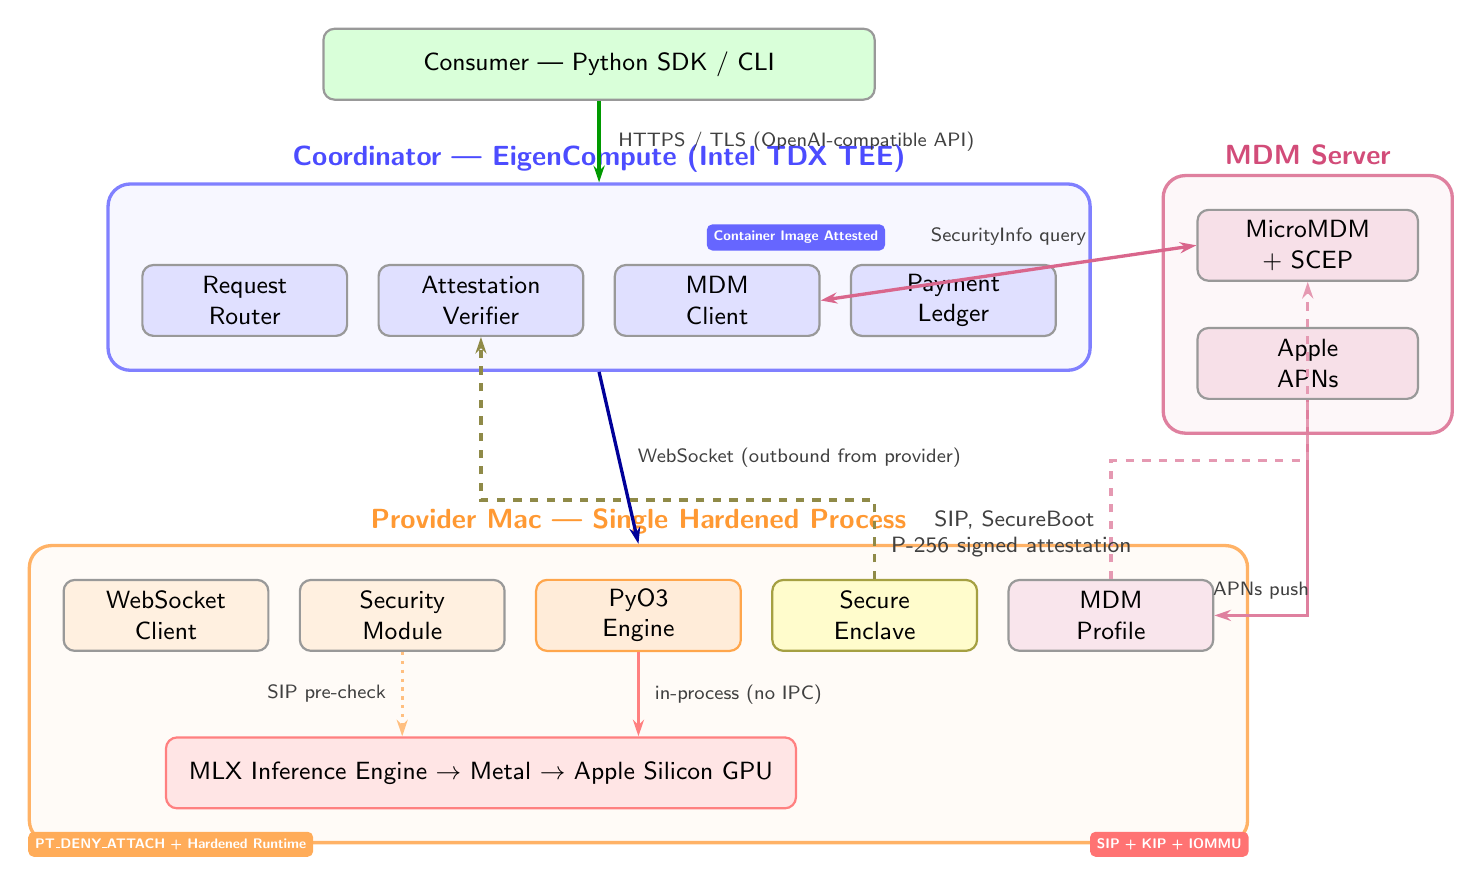
\begin{tikzpicture}[
    component/.style={draw=gray!80, thick, rounded corners=4pt, fill=#1, minimum width=2.6cm, minimum height=0.9cm, font=\small\sffamily, align=center},
    component/.default={white},
    groupbox/.style={draw=#1, very thick, rounded corners=8pt, inner sep=12pt},
    groupbox/.default={gray!50},
    arr/.style={-{Stealth[length=6pt,width=4pt]}, very thick, #1},
    arr/.default={gray!60},
    biarr/.style={{Stealth[length=6pt,width=4pt]}-{Stealth[length=6pt,width=4pt]}, very thick, #1},
    biarr/.default={gray!60},
    lbl/.style={font=\scriptsize\sffamily, #1},
    lbl/.default={gray!50!black},
    grouptitle/.style={font=\normalsize\sffamily\bfseries, #1},
    grouptitle/.default={black},
    badge/.style={font=\tiny\sffamily\bfseries, rounded corners=2pt, fill=#1, text=white, inner sep=2.5pt},
]

\node[component=green!15, minimum width=7cm] (consumer) at (0, 0) {Consumer --- Python SDK / CLI};

\node[component=blue!12] (router) at (-4.5, -3) {Request\\Router};
\node[component=blue!12] (attverify) at (-1.5, -3) {Attestation\\Verifier};
\node[component=blue!12] (mdmclient) at (1.5, -3) {MDM\\Client};
\node[component=blue!12] (payments) at (4.5, -3) {Payment\\Ledger};
\node[minimum height=0.5cm, minimum width=1cm] (coordspacer) at (4.5, -2.2) {};
\begin{scope}[on background layer]
\node[groupbox=blue!50, fill=blue!3, fit=(router)(attverify)(mdmclient)(payments)(coordspacer),
      label={[grouptitle=blue!70]above:{Coordinator --- EigenCompute (Intel TDX TEE)}}] (coordbox) {};
\end{scope}
\node[badge=blue!60] at (2.5, -2.2) {Container Image Attested};

\node[component=purple!12, minimum width=2.8cm] (mdmserver) at (9, -2.3) {MicroMDM\\+ SCEP};
\node[component=purple!12, minimum width=2.8cm] (apns) at (9, -3.8) {Apple\\APNs};
\begin{scope}[on background layer]
\node[groupbox=purple!50, fill=purple!3, fit=(mdmserver)(apns),
      label={[grouptitle=purple!70]above:{MDM Server}}] (mdmbox) {};
\end{scope}

\node[component=orange!12] (wsclient) at (-5.5, -7) {WebSocket\\Client};
\node[component=orange!12] (secmod) at (-2.5, -7) {Security\\Module};
\node[component=orange!15, draw=orange!70] (pyo3eng) at (0.5, -7) {PyO3\\Engine};
\node[component=yellow!20, draw=yellow!60!black] (secenclave) at (3.5, -7) {Secure\\Enclave};
\node[component=red!10, draw=red!50, minimum width=8cm, minimum height=0.9cm]
    (mlxgpu) at (-1.5, -9) {MLX Inference Engine $\to$ Metal $\to$ Apple Silicon GPU};
\node[component=purple!10] (mdmprof) at (6.5, -7) {MDM\\Profile};
\begin{scope}[on background layer]
\node[groupbox=orange!60, fill=orange!3, fit=(wsclient)(secmod)(pyo3eng)(secenclave)(mlxgpu)(mdmprof),
      label={[grouptitle=orange!80]above:{Provider Mac --- Single Hardened Process}}] (provbox) {};
\end{scope}
\node[badge=orange!65, anchor=west] at (provbox.south west) {PT\_DENY\_ATTACH + Hardened Runtime};
\node[badge=red!55, anchor=east] at (provbox.south east) {SIP + KIP + IOMMU};

% ===== ARROWS =====
\draw[arr=green!60!black] (consumer.south) -- (coordbox.north) node[lbl, midway, right=3pt] {HTTPS / TLS (OpenAI-compatible API)};
\draw[arr=blue!60!black] (coordbox.south) -- (provbox.north) node[lbl, midway, right=3pt] {WebSocket (outbound from provider)};
\draw[biarr=purple!60] (mdmclient.east) -- (mdmserver.west) node[lbl, midway, above=6pt] {SecurityInfo query};
\draw[arr=purple!50] (apns.south) |- (mdmprof.east) node[lbl, pos=0.75, above=2pt] {APNs push};
\draw[arr=purple!40, dashed] (mdmprof.north) -- ++(0, 1.5) node[lbl, left=2pt, pos=0.5] {\footnotesize SIP, SecureBoot} -| (mdmserver.south);
\draw[arr=yellow!50!black, dashed] (secenclave.north) -- ++(0, 1.0) node[lbl, right=2pt, pos=0.4] {\footnotesize P-256 signed attestation} -| (attverify.south);
\draw[arr=red!50] (pyo3eng.south) -- (mlxgpu.north-|pyo3eng.south) node[lbl, midway, right=2pt] {in-process (no IPC)};
\draw[arr=orange!50, dotted] (secmod.south) -- (mlxgpu.north-|secmod.south) node[lbl, midway, left=2pt] {SIP pre-check};

% Security Module annotations

\end{tikzpicture}
\caption{Complete DGInf system architecture. The consumer connects via HTTPS. The coordinator runs on EigenCompute (Intel TDX TEE) with cryptographic container attestation. The provider Mac runs all inference in a single hardened process protected by PT\_DENY\_ATTACH, Hardened Runtime, SIP, KIP, and IOMMU. The Secure Enclave provides hardware-bound P-256 identity. The MDM server independently verifies security posture (SIP, Secure Boot) via Apple APNs, cross-checked against the provider's self-reported attestation.}
\label{fig:arch}
\end{figure*}

\subsection{In-Process Inference via PyO3}

Traditional inference serving architectures (vLLM, Ollama, llama.cpp server) run the engine as a separate HTTP server process. This creates two attack surfaces: (a)~localhost TCP traffic can be captured via \texttt{tcpdump}, which functions even with SIP enabled; and (b)~the server binary can be modified to log all requests.

DGInf eliminates both by embedding the Python MLX inference engine directly in the Rust provider process using PyO3~\cite{pyo3}:

\begin{lstlisting}[language=Python,caption={Inference runs inside the hardened Rust process---no subprocess, no HTTP, no socket.}]
# Executed inside Rust process via PyO3
import mlx_lm, builtins

# Load model in-process
builtins._model, builtins._tok = \
    mlx_lm.load("Qwen3.5-9B-MLX-4bit")

# All inference in hardened process memory
result = mlx_lm.generate(
    builtins._model, builtins._tok,
    prompt=prompt, max_tokens=256)
\end{lstlisting}

The Python interpreter, model weights (potentially 76\,GB for Qwen3.5-122B at Q4), tokenizer, and all intermediate computation reside in a single process address space. This space is protected by three kernel-enforced mechanisms:

\begin{enumerate}[leftmargin=*,itemsep=1pt,topsep=2pt]
    \item \textbf{\texttt{PT\_DENY\_ATTACH}} (ptrace constant 31): Called at process startup before any sensitive data is loaded. Instructs the macOS kernel to permanently deny all \texttt{ptrace} requests against this process, including from root. This blocks lldb, dtrace, and Instruments.
    \item \textbf{Hardened Runtime}: The binary is code-signed with \texttt{-{}-options runtime} and explicitly \emph{without} the \texttt{com.apple.security.get-task-allow} entitlement. This causes the kernel to deny \texttt{task\_for\_pid()} and \texttt{mach\_vm\_read()} from any external process---the standard macOS APIs for reading another process's memory.
    \item \textbf{SIP enforcement}: System Integrity Protection enforces both of the above at the kernel level. With SIP enabled, even root cannot circumvent Hardened Runtime protections or load unsigned kernel extensions.
\end{enumerate}

\subsection{Python Path Locking}

A subtle attack: the provider installs a malicious \texttt{mlx-lm} package that logs all prompts. Since this code runs \emph{inside} our hardened process, PT\_DENY\_ATTACH would protect the attacker's code from inspection.

We prevent this by locking \texttt{sys.path} at initialization to only include packages from the signed application bundle, excluding system \texttt{site-packages}. Any modification to the bundle invalidates its code signature; SIP prevents macOS from executing binaries with invalid signatures.

\subsection{Memory Wiping}

After each inference request, buffers containing prompts and model outputs are zeroed using \texttt{write\_volatile} (prevents compiler dead store elimination) followed by a sequential-consistency memory fence.

\subsection{Secure Enclave Attestation}

On first run, the provider generates a P-256 ECDSA signing key inside Apple's Secure Enclave via CryptoKit. The private key never leaves the hardware---the \texttt{dataRepresentation} stored on disk is an opaque handle that only works on the device that created it. The provider constructs a signed attestation blob containing hardware identity, security posture, and cryptographic bindings:

\begin{table}[h]
\centering
\caption{Attestation blob fields. All fields are JSON-encoded with sorted keys (deterministic for signing) and signed by the Secure Enclave P-256 key.}
\vspace{4pt}
\scriptsize
\begin{tabular}{@{}llp{3.2cm}@{}}
\toprule
\textbf{Field} & \textbf{Example} & \textbf{Purpose} \\
\midrule
\texttt{chipName} & Apple M3 Max & Hardware identity \\
\texttt{hardwareModel} & Mac15,8 & Machine model \\
\texttt{osVersion} & 15.3.0 & macOS version \\
\texttt{serialNumber} & FV0FJ93J4D & MDM cross-reference (Section~5) \\
\texttt{publicKey} & (base64, 64\,B) & P-256 public key (raw X$\|$Y) \\
\texttt{encryptionPublicKey} & (base64, 32\,B) & X25519 key bound to this identity \\
\texttt{binaryHash} & (hex, 64 chars) & SHA-256 of provider binary \\
\texttt{sipEnabled} & true & SIP status (software check) \\
\texttt{secureBootEnabled} & true & Secure Boot status \\
\texttt{secureEnclaveAvailable} & true & SE hardware present \\
\texttt{authenticatedRootEnabled} & true & Sealed system volume (ARV) \\
\texttt{systemVolumeHash} & (hex, 64 chars) & APFS snapshot hash of system volume \\
\texttt{timestamp} & ISO 8601 & Freshness \\
\bottomrule
\end{tabular}
\end{table}

The blob is JSON-encoded with \texttt{.sortedKeys} to produce deterministic output, then signed with the Secure Enclave key. The result is a \texttt{SignedAttestation} containing the blob plus a base64 DER-encoded ECDSA signature.

Three fields deserve special attention:

\textbf{serialNumber.}\quad The hardware serial number enables the coordinator to look up the device in the MDM server and independently verify its security posture (Section~5). Without this field, MDM cross-verification would be impossible.

\textbf{binaryHash.}\quad The SHA-256 hash of the running \texttt{dginf-provider} binary. The coordinator maintains a list of blessed binary hashes for each release. If the hash does not match, the provider is running modified code and is rejected. This prevents a provider from patching the binary to bypass security checks (e.g., removing the SIP verification or the Python path locking).

\textbf{encryptionPublicKey.}\quad Binds the provider's X25519 encryption key (used for future end-to-end encrypted inference) to the same Secure Enclave identity. The coordinator verifies this matches the public key in the registration message, proving the same physical device controls both keys.

\textbf{authenticatedRootEnabled.}\quad Reports whether the Authenticated Root Volume (ARV) is active, checked via \texttt{csrutil authenticated-root status}. ARV seals the macOS system volume with a Merkle tree of SHA-256 hashes. Any modification to any system file (including \texttt{mdmclient}, \texttt{csrutil}, kernel caches) breaks the seal and prevents the volume from mounting. This is a stronger guarantee than SIP alone: SIP prevents \emph{runtime} modifications, while ARV proves the \emph{entire system volume} is Apple's original, unmodified build.

\textbf{systemVolumeHash.}\quad The cryptographic hash of the APFS system volume snapshot (extracted from \texttt{diskutil info /}). This hash uniquely identifies the exact macOS build running on the device. The coordinator can cross-reference this hash against known-good macOS builds published by Apple, detecting providers running modified or outdated operating systems. Combined with ARV, this provides two independent proofs of system volume integrity.

\subsubsection{Signature Verification}

The coordinator verifies the attestation by:
\begin{enumerate}[leftmargin=*,itemsep=1pt]
    \item Decoding the P-256 public key from the blob (64-byte raw X$\|$Y format)
    \item Hashing the original JSON blob bytes with SHA-256
    \item Verifying the DER-encoded ECDSA signature against the hash
    \item Checking: SE available? SIP enabled? Secure Boot enabled? ARV enabled?
    \item Checking: \texttt{encryptionPublicKey} matches registration key?
    \item Checking: \texttt{binaryHash} matches a known blessed version?
    \item If all pass $\to$ proceed to MDM verification (Section~5)
\end{enumerate}

A critical implementation detail: Swift's \texttt{JSONEncoder} with \texttt{.sortedKeys} produces alphabetically-ordered JSON keys. The Go coordinator must produce identical byte-for-byte JSON for signature verification. We achieve this by declaring Go struct fields in alphabetical order by JSON tag name, with a \texttt{marshalSortedJSON} fallback that uses a \texttt{map[string]interface\{\}} (Go 1.12+ marshals map keys in sorted order).

\subsubsection{Cross-Language Compatibility}

The attestation protocol spans three languages: Swift (Secure Enclave signing), Rust (provider agent), and Go (coordinator verification). All three must produce identical JSON representations of the attestation blob for signatures to verify. We enforce this through:
\begin{itemize}[leftmargin=*,itemsep=1pt]
    \item Alphabetically-ordered struct fields in all three languages
    \item \texttt{omitempty} / optional handling: nil fields are omitted (not null)
    \item ISO 8601 timestamp format with consistent precision
    \item Base64 encoding with standard alphabet (no URL-safe variant)
    \item Raw P-256 public key format (64 bytes: X$\|$Y, no 0x04 prefix)
\end{itemize}

% =====================================================================
\section{Formal Security Model}

\subsection{Actors and Assumptions}

\begin{definition}[Trust Model]
\label{def:trust}
We define four actors:
\begin{itemize}[leftmargin=*,itemsep=1pt,topsep=2pt]
    \item $\mathcal{C}$ (Consumer): Trusted. Initiates requests and verifies provider attestation.
    \item $\mathcal{K}$ (Coordinator): Trusted via hardware. Runs on EigenCompute~\cite{eigencloud} (Intel TDX TEE on GCP). The container image is cryptographically attested---consumers can verify the coordinator code is unmodified. Even DGInf as a company cannot read coordinator memory.
    \item $\mathcal{P}$ (Provider): \textbf{Untrusted and adversarial.} Owns the Mac hardware, has root access, and may actively attempt to read inference data.
    \item $\mathcal{A}$ (Apple): Trusted for correctness of: Secure Enclave, SIP implementation, Kernel Integrity Protection, Hardened Runtime enforcement, IOMMU policy, and code signature verification.
\end{itemize}
\end{definition}

\begin{definition}[Threat Model]
The adversary $\mathcal{P}$ can:
\begin{itemize}[leftmargin=*,itemsep=1pt]
    \item Execute arbitrary code as root on the Mac
    \item Install any software (subject to SIP restrictions)
    \item Reboot the machine at any time
    \item Physically access the machine
\end{itemize}
The adversary $\mathcal{P}$ \emph{cannot}:
\begin{itemize}[leftmargin=*,itemsep=1pt]
    \item Exploit unpatched kernel vulnerabilities (Assumption~\ref{asm:kernel})
    \item Modify Secure Enclave firmware
    \item Desolder LPDDR5x memory from the SoC package without destroying it
\end{itemize}
\end{definition}

\begin{definition}[Assumptions]
\label{asm:kernel}
\textbf{Assumption 1} (Kernel Integrity): The macOS kernel has no unpatched vulnerabilities that allow SIP bypass, Hardened Runtime bypass, or KIP circumvention. This is a standard assumption in systems security---Apple has patched all known SIP bypass CVEs (e.g., CVE-2022-22583, CVE-2022-42821, CVE-2023-32369) within weeks of disclosure.

\textbf{Assumption 2} (Secure Enclave Integrity): The Secure Enclave hardware and firmware correctly implement key generation, signing, and isolation. This is a hardware trust assumption analogous to trusting Intel SGX or ARM TrustZone.
\end{definition}

\subsection{Attack Surface Analysis}

Table~\ref{tab:attacks} enumerates all software-based attacks against the provider process and their corresponding defenses.

\begin{table*}[t]
\centering
\caption{Complete software attack surface on Apple Silicon. All listed attacks are blocked under Assumptions 1--2.}
\label{tab:attacks}
\vspace{4pt}
\small
\begin{tabularx}{\textwidth}{@{}lXl@{}}
\toprule
\textbf{Attack Vector} & \textbf{Defense} & \textbf{Enforced By} \\
\midrule
Attach debugger (lldb, dtrace, Instruments) & \texttt{ptrace(PT\_DENY\_ATTACH)} at process startup & Kernel \\
Read memory via Mach APIs (task\_for\_pid, mach\_vm\_read) & Hardened Runtime: no \texttt{get-task-allow} entitlement & Kernel \\
Sniff IPC between provider and inference engine & No IPC channel exists---all inference is in-process via PyO3 & Architecture \\
Modify provider binary to add logging & Code signing + SIP: macOS refuses to execute modified signed binaries & Kernel + SIP \\
Replace binary with malicious version & Binary SHA-256 included in Secure Enclave-signed attestation; coordinator rejects mismatches & Coordinator \\
Inject malicious Python package (e.g., trojan mlx-lm) & \texttt{sys.path} locked to signed app bundle; system site-packages excluded & Process + SIP \\
Load unsigned kernel extension for memory access & SIP blocks all unsigned kernel extensions on Apple Silicon & SIP \\
Modify kernel code at runtime & Kernel Integrity Protection (KIP): memory controller hardware denies writes to kernel pages after boot & Hardware \\
Disable SIP to bypass all software protections & Requires reboot into Recovery Mode, terminating all processes (Theorem~\ref{thm:sip}) & Hardware \\
Read physical memory via \texttt{/dev/mem} & Device node does not exist on Apple Silicon & Hardware \\
DMA-based memory extraction via Thunderbolt/PCIe & Per-device IOMMU with default-deny policy; unauthorized DMA triggers kernel panic & Hardware \\
\midrule
\textit{Physical memory probing} & \textit{LPDDR5x soldered into SoC package; desoldering is destructive} & \textit{Physical} \\
\bottomrule
\end{tabularx}
\end{table*}

\subsection{SIP Runtime Immutability}

The security of our architecture depends on the claim that SIP, once verified at process startup, cannot be disabled during the process lifetime. We formalize this:

\begin{lemma}[SIP State Persistence]
\label{lem:sip-nvram}
SIP state $S \in \{\textsc{enabled}, \textsc{disabled}\}$ is stored in NVRAM and is immutable to all userspace code, including code running as root, in the normal macOS boot environment.
\end{lemma}

\begin{proof}
The SIP state variable is stored in the machine's NVRAM (non-volatile random-access memory) and is read by the Boot ROM during the secure boot chain. The only utility that modifies this variable is \texttt{csrutil}, which Apple restricts to execution within the Recovery Mode boot environment $\mathcal{R}$. When running in the normal macOS environment, \texttt{csrutil disable} returns an error. No other userspace or kernel API exposes write access to the SIP NVRAM variable when SIP is enabled, as SIP itself protects the NVRAM variables that control it (a self-reinforcing property).
\end{proof}

\begin{theorem}[SIP Runtime Immutability]
\label{thm:sip}
Under Assumption~1 (no unpatched kernel vulnerabilities), if SIP is verified as enabled at process startup time $t_0$, then SIP remains enabled at all times $t \in [t_0, t_{\text{end}}]$ during the lifetime of that process.
\end{theorem}

\begin{proof}
By Lemma~\ref{lem:sip-nvram}, SIP state is immutable in the normal boot environment. The only mechanism to change SIP state is:
\begin{enumerate}[leftmargin=*,itemsep=1pt]
    \item Reboot into Recovery Mode environment $\mathcal{R}$
    \item Execute \texttt{csrutil disable} in $\mathcal{R}$
    \item Reboot back to the normal environment
\end{enumerate}

Step 1 requires a hardware reboot. Let $\mathcal{E}(t)$ denote the set of all running processes at time $t$. A reboot at time $t_r$ terminates every process:
\begin{equation}
    \forall\, p \in \mathcal{E}(t_r^-):\; \lnot\,\text{alive}(p,\, t_r^+)
\end{equation}

The DGInf provider process $p^* \in \mathcal{E}(t_0)$. If $p^*$ verified $S(t_0) = \textsc{enabled}$, then for $p^*$ to observe $S = \textsc{disabled}$, a reboot must occur. But a reboot terminates $p^*$. Therefore, during the lifetime of $p^*$:
\begin{equation}
    S(t_0) = \textsc{enabled} \;\implies\; \forall\, t \in [t_0,\, t_{\text{end}}]:\; S(t) = \textsc{enabled}
\end{equation}

\textbf{Note on Assumption~1:} Without this assumption, a kernel vulnerability could theoretically allow direct NVRAM modification from the normal environment, bypassing both SIP's self-protection and the Recovery Mode requirement. Apple has patched all known such vulnerabilities (CVE-2022-22583, CVE-2022-42821, CVE-2023-32369). The assumption is that the current kernel has no \emph{unpatched} vulnerability of this class.
\end{proof}

\begin{corollary}[Single Check Sufficiency]
A single SIP verification at process startup provides a security guarantee for the entire process lifetime. Pre-request SIP checks serve as defense-in-depth but cannot detect a state change (because none can occur under the theorem's assumptions).
\end{corollary}

\subsection{Provider Verification Requirements}

\begin{definition}[Verified Provider]
A provider is \emph{verified} if and only if all of the following hold:
\begin{enumerate}[leftmargin=*,itemsep=1pt]
    \item Secure Enclave P-256 attestation signature is valid
    \item Binary hash matches a known blessed version
    \item Device is enrolled in DGInf MDM
    \item MDM SecurityInfo confirms: SIP enabled, Secure Boot ``full,'' Authenticated Root Volume enabled, and system volume hash matches a known-good macOS build
    \item MDM-reported posture matches self-reported attestation (no discrepancies)
    \item Periodic challenge-response includes fresh SIP and Secure Boot status
\end{enumerate}
Unverified providers receive no jobs. There is no degraded mode---the network requires hardware-verified trust from every provider. If any check fails or any discrepancy is detected between MDM and self-reported posture, the provider is rejected immediately.
\end{definition}

\subsection{Comparison with Apple PCC}

\begin{table}[h]
\centering
\caption{DGInf vs.\ Apple Private Cloud Compute.}
\label{tab:pcc}
\vspace{4pt}
\small
\begin{tabular}{@{}lcc@{}}
\toprule
\textbf{Property} & \textbf{Apple PCC} & \textbf{DGInf} \\
\midrule
Hardware owner & Trusted (Apple) & Adversarial \\
Physical security & Guards + tamper & Soldered LPDDR5x \\
Coordinator TEE & N/A (Apple infra) & EigenCompute (TDX) \\
OS immutability & SSV & SIP + ARV + SSV hash \\
Shell/debug access & Removed entirely & Blocked at kernel \\
Memory encryption & None & None \\
Provider verification & Apple-signed & SE + MDM (mandatory) \\
Coordinator attest. & N/A & Container image hash \\
Remaining attack & Physical probing & Physical probing \\
\bottomrule
\end{tabular}
\end{table}

% =====================================================================
\section{MDM-Based Independent Verification}

\subsection{Motivation}

Secure Enclave attestation alone has two limitations: (a)~the coordinator cannot prove the P-256 signing key resides in the Secure Enclave rather than software (both produce identical ECDSA signatures); (b)~the SIP status in the attestation blob is obtained via \texttt{csrutil status}, which is a software check that could be spoofed by a compromised system. MDM verification is therefore \emph{mandatory}, not optional---it is the mechanism that closes both gaps.

We address both through \emph{independent verification}: the coordinator queries the device's security posture through Apple's MDM framework, which returns data from the OS MDM client---not from the DGInf provider software.

\subsection{SecurityInfo Verification}

Apple's MDM \texttt{SecurityInfo} command~\cite{apple-mdm} returns:

\begin{table}[h]
\centering
\small
\begin{tabular}{@{}ll@{}}
\toprule
\textbf{Field} & \textbf{Meaning} \\
\midrule
\texttt{SIPEnabled} & System Integrity Protection \\
\texttt{SecureBootLevel} & full / reduced / permissive \\
\texttt{AuthRootVolume} & Signed System Volume \\
\texttt{FDE\_Enabled} & FileVault encryption \\
\texttt{RecoveryLock} & Recovery Mode password \\
\bottomrule
\end{tabular}
\end{table}

\textbf{Self-reinforcing security argument:} Spoofing the MDM response requires modifying system frameworks (\texttt{/System/Library/}), which requires SIP to be disabled. But SIP being disabled is precisely what the MDM check detects. Thus, a provider cannot spoof the SIP check without the genuine check revealing SIP is disabled.

More importantly, the security model is \emph{self-reinforcing}: the only scenario where SecurityInfo can be spoofed (SIP disabled) is exactly the scenario where the provider can already read inference data from memory via debuggers, \texttt{task\_for\_pid}, or kernel extensions. Spoofing SecurityInfo gains the attacker nothing they don't already have. This circular dependency, combined with Authenticated Root Volume verification (which proves the entire system volume is Apple's sealed, unmodified build), creates a multi-layered guarantee where each layer independently verifies the others.

We further strengthen this with the \texttt{systemVolumeHash}: the APFS snapshot hash uniquely identifies the exact macOS build. Even if a provider somehow spoofed SecurityInfo while keeping SIP enabled, the system volume hash would not match known-good Apple builds if any system binary had been modified.

\subsection{Verification Flow}

\begin{figure}[t]
\centering
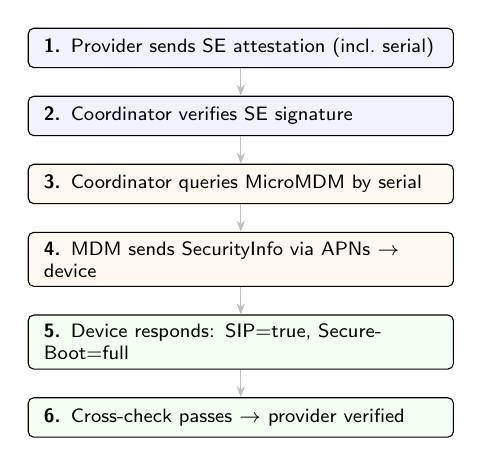
\begin{tikzpicture}[
    node distance=0.35cm,
    step/.style={draw, rounded corners=2pt, fill=#1, minimum width=5.4cm, minimum height=0.5cm, font=\scriptsize\sffamily, align=left, text width=5.0cm},
]
    \node[step=blue!5] (s1) {\textbf{1.} Provider sends SE attestation (incl.\ serial)};
    \node[step=blue!5, below=of s1] (s2) {\textbf{2.} Coordinator verifies SE signature};
    \node[step=orange!5, below=of s2] (s3) {\textbf{3.} Coordinator queries MicroMDM by serial};
    \node[step=orange!5, below=of s3] (s4) {\textbf{4.} MDM sends SecurityInfo via APNs $\to$ device};
    \node[step=green!5, below=of s4] (s5) {\textbf{5.} Device responds: SIP=true, SecureBoot=full};
    \node[step=green!5, below=of s5] (s6) {\textbf{6.} Cross-check passes $\to$ provider verified};

    \foreach \a/\b in {s1/s2, s2/s3, s3/s4, s4/s5, s5/s6} {
        \draw[-{Stealth[length=4pt]}, gray!50] (\a.south) -- (\b.north);
    }
\end{tikzpicture}
\caption{MDM verification flow. The coordinator independently queries Apple's MDM framework, then cross-checks against the provider's self-reported attestation. Discrepancies cause immediate trust revocation.}
\label{fig:mdm}
\end{figure}

\subsection{Enrollment and Permissions}

A core design goal is that MDM enrollment must be \emph{non-invasive}---the provider should not feel that DGInf has control over their Mac. Apple's MDM protocol uses a bitmask called \texttt{AccessRights} to define exactly what the MDM server can do. Each bit grants a specific capability:

\begin{table}[h]
\centering
\caption{Apple MDM AccessRights bitmask. DGInf requests only bits 0, 4, and 10 (bold).}
\label{tab:accessrights}
\vspace{4pt}
\scriptsize
\begin{tabular}{@{}rlcc@{}}
\toprule
\textbf{Bit} & \textbf{Permission} & \textbf{DGInf} & \textbf{Typical MDM} \\
\midrule
\textbf{0} & \textbf{Inspect device} & \checkmark & \checkmark \\
1 & Install/remove configuration profiles & --- & \checkmark \\
2 & Device lock and passcode removal & --- & \checkmark \\
3 & \textcolor{red}{Erase all data on device} & --- & \checkmark \\
\textbf{4} & \textbf{Query device information} & \checkmark & \checkmark \\
5 & Query network information & --- & \checkmark \\
6 & Inspect provisioning profiles & --- & \checkmark \\
7 & Install/remove provisioning profiles & --- & \checkmark \\
8 & Inspect installed applications & --- & \checkmark \\
9 & Restriction-related queries & --- & \checkmark \\
\textbf{10} & \textbf{Query security information} & \checkmark & \checkmark \\
11 & Change device settings & --- & \checkmark \\
12 & App management & --- & \checkmark \\
\bottomrule
\end{tabular}
\end{table}

DGInf requests \texttt{AccessRights\,=\,1041} ($2^0 + 2^4 + 2^{10}$), granting \emph{only} three capabilities:
\begin{itemize}[leftmargin=*,itemsep=1pt]
    \item \textbf{Bit 0}: Inspect device (basic query capability)
    \item \textbf{Bit 4}: Query device information (model, OS version, serial)
    \item \textbf{Bit 10}: Query security information (\texttt{SecurityInfo} command)
\end{itemize}

The remaining 10 bits are explicitly \emph{not set}. The MDM server \textbf{cannot}: erase the device, lock it, change the passcode, install or remove profiles, install or remove apps, modify settings, query network details, or inspect installed applications. This is verified by macOS itself when the enrollment profile is installed---the system displays the exact permissions to the user before they consent.

Providers can \textbf{unenroll at any time} from System Settings $\to$ General $\to$ Device Management by removing the profile. Unenrollment is instant and complete.

\subsection{SecurityInfo: What MDM Returns}

The \texttt{SecurityInfo} command returns the following fields, verified by the OS MDM framework:

\begin{table}[h]
\centering
\caption{Fields returned by the MDM \texttt{SecurityInfo} command.}
\vspace{4pt}
\small
\begin{tabular}{@{}lp{4.5cm}@{}}
\toprule
\textbf{Field} & \textbf{What It Proves} \\
\midrule
\texttt{SIPEnabled} & System Integrity Protection is on---root cannot modify /System or bypass Hardened Runtime \\
\texttt{SecureBootLevel} & Boot security: ``full'' means only Apple-signed code runs at boot \\
\texttt{AuthRootVolume} & Signed System Volume is intact (Merkle tree verified) \\
\texttt{FDE\_Enabled} & FileVault disk encryption is active \\
\texttt{RecoveryLock} & Recovery Mode requires a password (prevents casual SIP disable) \\
\texttt{FirewallEnabled} & Application firewall is active \\
\texttt{RemoteDesktop} & Screen Sharing / ARD is active \\
\bottomrule
\end{tabular}
\end{table}

For DGInf, the critical fields are \texttt{SIPEnabled} (must be true for all our kernel-level protections to hold), \texttt{SecureBootLevel} (must be ``full''), and \texttt{AuthRootVolume} (ensures the OS hasn't been tampered with).

\subsection{Apple Device Attestation (MDA)}

After SecurityInfo verification, the coordinator requests \texttt{DevicePropertiesAttestation} via the MDM \texttt{DeviceInformation} command. The device contacts Apple's attestation servers, which return a DER-encoded X.509 certificate chain:

\begin{itemize}[leftmargin=*,itemsep=1pt]
    \item \textbf{Leaf certificate}: Device identity with Apple-assigned OIDs encoding the serial number (1.2.840.113635.100.8.9.1), UDID (100.8.9.2), OS version (100.8.10.1), SepOS version (100.8.10.2), and Secure Boot level (100.8.13.2).
    \item \textbf{Intermediate}: Apple Enterprise Attestation Sub CA~1 (P-384).
    \item \textbf{Root}: Apple Enterprise Attestation Root CA (P-384, valid until 2047).
\end{itemize}

This is the strongest verification available: Apple's own servers cryptographically attest the device's identity and security properties. A compromised OS cannot forge this certificate chain---the private key for Apple's root CA exists only inside Apple's infrastructure.

The coordinator verifies the chain against the embedded Apple root CA, extracts the OID-encoded properties, and cross-checks the serial number against the provider's self-reported attestation. The full certificate chain is stored and exposed via \texttt{GET /v1/providers/attestation}, enabling users to independently verify each provider against Apple's publicly available root CA.

\subsection{Challenge-Response with SIP Re-Verification}

Every 5 minutes, the coordinator sends a 32-byte nonce. The provider signs it and includes \emph{fresh} SIP and Secure Boot status. If either is reported as disabled, the provider is \textbf{immediately} marked untrusted---no three-strike rule, because disabled SIP or Secure Boot indicates a deliberate reboot with weakened security.

This catches the scenario where a provider: (a)~registers with SIP enabled, (b)~reboots into Recovery Mode and disables SIP, (c)~reboots back and reconnects. The reconnection triggers a new registration with SIP=false in the attestation, and even if the provider lies, the next MDM SecurityInfo query independently reveals SIP=false.

% =====================================================================
\section{Implementation}

The complete implementation is open-source~\cite{dginf-repo}. The coordinator runs on EigenCompute~\cite{eigencloud}, Eigen Labs' verifiable cloud platform. EigenCompute provides Intel TDX hardware TEEs on GCP with cryptographic attestation of the deployed Docker container image. Consumers can verify that the coordinator is running the exact, unmodified DGInf code---DGInf as a company cannot tamper with the coordinator or access its memory.

The system comprises approximately 14,000 lines of code across five languages:

\begin{table}[h]
\centering
\caption{Implementation summary.}
\vspace{4pt}
\small
\begin{tabular}{@{}llr@{}}
\toprule
\textbf{Component} & \textbf{Language} & \textbf{LoC} \\
\midrule
Provider Agent & Rust & 4,500 \\
Coordinator & Go & 4,000 \\
Consumer Web Frontend & TypeScript (Next.js) & 2,500 \\
Consumer SDK & Python & 1,200 \\
Secure Enclave module & Swift & 600 \\
macOS App (GUI) & Swift/SwiftUI & 1,500 \\
\midrule
\textbf{Total} && \textbf{$\sim$14,300} \\
\bottomrule
\end{tabular}
\end{table}

Provider onboarding is a single command that downloads a self-contained bundle ($\sim$107\,MB) including the provider binary, Secure Enclave CLI, and a bundled Python 3.12 environment with vllm-mlx and all dependencies. No system Python, pip, or Homebrew is required:

\begin{lstlisting}[caption={One-command provider setup.}]
$ curl -fsSL https://dginf.io/install.sh | bash

  DGInf -- Decentralized Private Inference

  Apple M4 Max, 48GB, macOS 26.3
  Downloading DGInf (~107MB)...
  vllm-mlx 0.2.5
  Secure Enclave (fresh key)

  Ready! Start serving:
    dginf-provider serve

$ dginf-provider serve --model Qwen3.5-9B-MLX-4bit

  SIP enabled, Secure Enclave available
  Backend ready, connected to coordinator
\end{lstlisting}

% =====================================================================
\section{Evaluation}

\subsection{End-to-End Validation}

We validated on two Apple Silicon Macs simultaneously: AWS \texttt{mac2-m2.metal} (Apple M2, 24\,GB, macOS 14.8.4) and an M4 Max (48\,GB, macOS 26.3):

\begin{enumerate}[leftmargin=*,itemsep=1pt]
    \item Both providers enrolled in MDM (AccessRights=1041: query-only, no erase/lock/install)
    \item Both generated Secure Enclave attestation (serials: FV0FJ93J4D, F46GTCP40H)
    \item Coordinator verified SE signatures $\to$ \texttt{self\_signed} trust
    \item Coordinator queried MicroMDM; SecurityInfo confirmed SIP=true, SecureBoot=full, AuthenticatedRootVolume=true for both $\to$ \texttt{hardware} trust
    \item Coordinator requested \texttt{DevicePropertiesAttestation} via MDM; Apple's servers returned DER certificate chains signed by Apple Enterprise Attestation Root CA for both devices $\to$ \texttt{mda\_verified}
    \item Apple certificate chains verified against embedded root CA; serial numbers cross-checked against attestation blobs
    \item Two simultaneous consumer requests routed to both providers (health-aware scoring with concurrent batching)
    \item M4 Max: 92\,tok/s streaming (Qwen3.5 9B); M2: 22\,tok/s. 6,517 tokens generated in 76.2\,s with zero errors
    \item 8 concurrent requests completed with 100\% success rate across both providers
    \item Consumer disconnect triggered cancel propagation: coordinator $\to$ provider $\to$ HTTP connection dropped $\to$ backend stopped generating within 1\,s
    \item Full attestation proof exposed at \texttt{GET /v1/providers/attestation} for independent user verification against Apple's public Enterprise Attestation Root CA
\end{enumerate}

\subsection{Security and Performance}

\begin{table}[h]
\centering
\caption{Security verification and performance on two providers (M4 Max + M2).}
\vspace{4pt}
\small
\begin{tabular}{@{}ll|lr@{}}
\toprule
\textbf{Security Check} & \textbf{Result} & \textbf{Performance} & \textbf{Value} \\
\midrule
PT\_DENY\_ATTACH & lldb denied & Streaming (9B, M4 Max) & 92\,tok/s \\
SIP status & Enabled & Streaming (9B, M2) & 22\,tok/s \\
Secure Boot & Full & Time to first token & 1.4\,s \\
Auth Root Volume & Enabled & Reconnect after restart & $<$1\,s \\
MDM SecurityInfo & Match & Concurrent requests & 4/provider \\
Apple MDA cert chain & Verified & 8 concurrent, 0 failures & 100\% \\
Provider trust & \texttt{hardware} & SIP check & 12\,ms \\
\bottomrule
\end{tabular}
\end{table}

Security overhead is negligible. The SIP check (12\,ms) is the largest per-request cost, dominated by spawning \texttt{csrutil status} as a subprocess. This could be eliminated by caching the result (justified by Theorem~\ref{thm:sip}).

% =====================================================================
\section{Economics of Decentralized Inference}

\subsection{Cost Model}

For providers with hardware already purchased, marginal cost per million output tokens is:
\begin{equation}
    C_{\text{local}} = \frac{P_{\text{elec}}}{R_{\text{tok}} \times 3{,}600} \times 10^6
\end{equation}
where $P_{\text{elec}}$ is electricity (\$/hr) and $R_{\text{tok}}$ is decode throughput (tok/s). At US average residential \$0.15/kWh, a Mac Studio draws $\sim$100\,W under load (\$0.015/hr) and 5\,W at idle (\$0.55/month).

\subsection{Throughput on Apple Silicon}

\begin{table}[h]
\centering
\caption{Decode throughput (tok/s, Q4 quantization) on Apple Silicon. $\dagger$\,=\,measured on live DGInf network; others bandwidth-scaled at 65\% efficiency.}
\vspace{4pt}
\small
\begin{tabular}{@{}llrrr@{}}
\toprule
\textbf{Model} & \textbf{Arch} & \textbf{M4 Max} & \textbf{M3 Ultra} \\
& & 546\,GB/s & 819\,GB/s \\
\midrule
Qwen3.5 9B & Dense & 92$\dagger$ & 94 \\
Qwen3.5 27B & Dense & 21 & 32 \\
Qwen3.5 35B-A3B & MoE (3B) & 101 & 152 \\
Llama 3.1 70B & Dense & 8 & 13 \\
Qwen3.5 122B-A10B & MoE (10B) & 25 & 35 \\
MiniMax M2.5 230B & MoE (10B) & --- & 40 \\
\bottomrule
\multicolumn{4}{@{}l}{\scriptsize ``---''\,=\,does not fit. Active params shown for MoE.}
\end{tabular}
\end{table}

\textbf{Key observation:} Qwen3.5~35B-A3B (MoE, 3B active) achieves 101\,tok/s on M4~Max---\emph{faster} than the dense Qwen3.5~27B at 21\,tok/s, despite being ``larger.'' For MoE models, only active expert weights traverse the memory bus per token.

\subsection{MoE: The Economic Sweet Spot}

\begin{figure}[t]
\centering
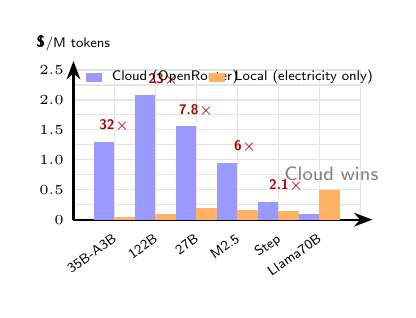
\begin{tikzpicture}[xscale=0.52, yscale=0.38]
    \draw[gray!20, thin] (0,0) grid[xstep=1,ystep=0.5] (7,5);
    \draw[-{Stealth}, thick] (0,0) -- (7.3,0);
    \draw[-{Stealth}, thick] (0,0) -- (0,5.3) node[above, font=\tiny\sffamily] {\$/M tokens};

    \foreach \y/\l in {0/0, 1/0.5, 2/1.0, 3/1.5, 4/2.0, 5/2.5} {
        \node[left, font=\tiny] at (0,\y) {\l};
    }

    \fill[blue!40] (0.5,0) rectangle (1.0,2.6);
    \fill[blue!40] (1.5,0) rectangle (2.0,4.16);
    \fill[blue!40] (2.5,0) rectangle (3.0,3.12);
    \fill[blue!40] (3.5,0) rectangle (4.0,1.9);
    \fill[blue!40] (4.5,0) rectangle (5.0,0.6);
    \fill[blue!40] (5.5,0) rectangle (6.0,0.2);

    \fill[orange!60] (1.0,0) rectangle (1.5,0.08);
    \fill[orange!60] (2.0,0) rectangle (2.5,0.18);
    \fill[orange!60] (3.0,0) rectangle (3.5,0.4);
    \fill[orange!60] (4.0,0) rectangle (4.5,0.32);
    \fill[orange!60] (5.0,0) rectangle (5.5,0.28);
    \fill[orange!60] (6.0,0) rectangle (6.5,0.98);

    \node[below, font=\tiny\sffamily, rotate=35, anchor=north east] at (1.0,0) {35B-A3B};
    \node[below, font=\tiny\sffamily, rotate=35, anchor=north east] at (2.0,0) {122B};
    \node[below, font=\tiny\sffamily, rotate=35, anchor=north east] at (3.0,0) {27B};
    \node[below, font=\tiny\sffamily, rotate=35, anchor=north east] at (4.0,0) {M2.5};
    \node[below, font=\tiny\sffamily, rotate=35, anchor=north east] at (5.0,0) {Step};
    \node[below, font=\tiny\sffamily, rotate=35, anchor=north east] at (6.0,0) {Llama70B};

    \node[above, font=\tiny\bfseries\sffamily, color=red!70!black] at (1.0,2.6) {32$\times$};
    \node[above, font=\tiny\bfseries\sffamily, color=red!70!black] at (2.2,4.16) {23$\times$};
    \node[above, font=\tiny\bfseries\sffamily, color=red!70!black] at (3.0,3.12) {7.8$\times$};
    \node[above, font=\tiny\bfseries\sffamily, color=red!70!black] at (4.2,1.9) {6$\times$};
    \node[above, font=\tiny\bfseries\sffamily, color=red!70!black] at (5.2,0.6) {2.1$\times$};
    \node[above, font=\tiny\sffamily, color=gray] at (6.3,0.98) {\scriptsize Cloud wins};

    \fill[blue!40] (0.3,4.6) rectangle (0.7,4.9);
    \node[right, font=\tiny\sffamily] at (0.7,4.75) {Cloud (OpenRouter)};
    \fill[orange!60] (3.3,4.6) rectangle (3.7,4.9);
    \node[right, font=\tiny\sffamily] at (3.7,4.75) {Local (electricity only)};
\end{tikzpicture}
\caption{Cost per million output tokens: cloud vs.\ local inference on Apple Silicon. MoE models with small active parameters are 6--32$\times$ cheaper locally. Dense 70B favors cloud due to bandwidth constraints.}
\label{fig:economics}
\end{figure}

Cloud providers price based on total parameter count (the ``branding'' number: 122B, 230B). Local inference cost depends only on \emph{active} parameters per token---typically 3--10B for MoE models. This creates dramatic savings (Figure~\ref{fig:economics}).

Conversely, dense models $>$32B favor cloud: H100 clusters with 3.35\,TB/s memory bandwidth are 6$\times$ faster than M4~Max (546\,GB/s) for bandwidth-bound decode.

\subsection{Marketplace Viability}

\begin{table}[h]
\centering
\caption{DGInf marketplace pricing creates value for both sides.}
\vspace{4pt}
\small
\begin{tabular}{@{}lrrrr@{}}
\toprule
\textbf{Model} & \textbf{Cloud} & \textbf{DGInf} & \textbf{Consumer} & \textbf{Provider} \\
& \$/M & \$/M & \textbf{saves} & \textbf{margin} \\
\midrule
Qwen3.5 122B & \$2.08 & \$0.80 & 62\% & 89\% \\
Qwen3.5 35B-A3B & \$1.30 & \$0.50 & 62\% & 92\% \\
MiniMax M2.5 & \$0.95 & \$0.50 & 47\% & 68\% \\
\bottomrule
\end{tabular}
\end{table}

At 50\% utilization, a Mac Studio M4~Max earns $\sim$\$141/month with 96\% margins. The Mac idles at 5\,W (\$0.55/month), making the opportunity cost of participation near zero.

% =====================================================================
\section{Beyond Inference: Private Decentralized Compute}

While this paper focuses on LLM inference, the security architecture we present---in-process execution, SIP immutability, Hardened Runtime, MDM verification, and signed application bundles---is not specific to inference. It provides a general-purpose framework for \emph{private decentralized compute} on Apple Silicon.

\subsection{Encrypted Model Execution}

A model builder could publish an encrypted model to the network. The model weights would be encrypted at rest, and the decryption key would only be released to providers whose security posture has been verified through the full trust chain (SE attestation + MDM verification + binary hash match). The provider's hardened process would decrypt the weights in memory, run inference, and wipe them after the job completes. The provider never sees the model weights in a form they can extract---the same protections that guard consumer prompts also guard model IP.

This enables a \textbf{model bounty} pattern: a model builder publishes an encrypted model with a reward for running it, and providers on the network compete to serve it. The model builder retains full IP protection without operating any infrastructure.

\subsection{General Private Compute}

The core insight---that SIP + Hardened Runtime + in-process execution creates an environment where the machine owner cannot inspect running computation---applies to any workload, not just inference:

\begin{itemize}[leftmargin=*,itemsep=2pt]
    \item \textbf{Fine-tuning on private data}: A data owner could send encrypted training data to a provider. The data is decrypted in the hardened process, used for fine-tuning, and wiped. The provider computes gradient updates without seeing the data.
    \item \textbf{Private evaluation}: Run benchmarks or evaluations on proprietary datasets without exposing the dataset to the compute provider.
    \item \textbf{Multi-party computation}: Multiple parties contribute encrypted inputs to a computation running on a verified provider. Each party's data is decrypted only in the hardened process.
    \item \textbf{Confidential data pipelines}: ETL, analytics, or ML feature engineering on sensitive data, executed on idle Macs with verified security posture.
\end{itemize}

In each case, the security guarantees are identical to those proven for inference: the provider cannot attach debuggers (PT\_DENY\_ATTACH), cannot read process memory (Hardened Runtime), cannot disable protections without rebooting (SIP immutability), and their security posture is independently verified (MDM). The coordinator, running on EigenCompute's Intel TDX TEE, orchestrates key release and job routing with cryptographic attestation of its own code.

This positions the network not merely as an inference marketplace, but as a \textbf{general-purpose private compute layer} built on consumer hardware---a decentralized alternative to cloud confidential computing that is 10--100$\times$ cheaper per node.

% =====================================================================
\section{Limitations and Future Work}

\subsection{Security Limitations}

We identify two fundamental security limitations that cannot be addressed by our architecture:

\textbf{Kernel vulnerabilities.}\quad Our security model (Theorem~\ref{thm:sip}) assumes no unpatched kernel vulnerabilities (Assumption~1). A macOS kernel 0-day could theoretically bypass SIP, Hardened Runtime, or KIP, undermining the entire trust model. This is an inherent limitation of any software-enforced security boundary---only hardware TEEs are immune to kernel-level attacks. We mitigate this through Apple's track record of rapid patching: all known SIP bypass CVEs have been addressed within weeks of disclosure. This is the strongest theoretical attack against our system.

\textbf{Timing side channels.}\quad It is important to distinguish between \emph{token content} and \emph{token timing}. Our architecture fully protects token content: the provider cannot see what tokens are being generated, because the inference process is protected by PT\_DENY\_ATTACH (no debugger), Hardened Runtime (no external memory reads), and in-process execution (no IPC to sniff). Tokens exist only in the hardened process memory and leave as encrypted WebSocket messages.

However, token \emph{timing} is observable. An observer monitoring network packet intervals can infer: approximate prompt length (from prefill duration), approximate response length (from number of output packets), and relative token generation difficulty (from inter-token delays). We do not implement constant-time inference, and no practical constant-time LLM implementation exists. Mitigations include response buffering (send in fixed-size batches at fixed intervals rather than streaming per-token) and random jitter. This limitation is shared with Apple PCC and all non-TEE inference systems.

\subsection{Upgradeable Components}

Several components have logical defenses today but could be strengthened:

\textbf{MDM attestation strength.}\quad Our MDM verification uses Apple's \texttt{SecurityInfo} command, which returns OS-level security posture data. Spoofing this requires SIP disabled, creating a circular dependency (Section~5.2) that serves as a logical defense. However, Managed Device Attestation (MDA) via Apple Business Manager would provide \emph{cryptographic} assurance: attestation certificates chain to Apple's Enterprise Root CA through the Secure Enclave, making spoofing impossible without compromising the Secure Enclave hardware itself. We have implemented the step-ca ACME infrastructure for MDA (\texttt{device-attest-01}); activation requires completing Apple Business Manager domain verification.

\textbf{Inference throughput.}\quad The embedded Python interpreter (PyO3) holds the Global Interpreter Lock during inference, serializing requests to one at a time. This is a performance limitation, not a security limitation. Direct Rust bindings to MLX's C++ API via \texttt{mlx-rs} would eliminate both the GIL bottleneck and the Python package injection attack surface entirely.

\subsection{Future Work}

\textbf{Encrypted model execution.}\quad The model bounty pattern (Section~9.1) requires a key management protocol where decryption keys are released only to verified providers. Architecturally straightforward but not yet implemented.

\textbf{Request anonymization.}\quad OHTTP (RFC~9458) relays and RSA blind signatures would prevent the coordinator from linking consumer identity to request content, achieving non-targetability (Apple PCC's fourth principle).

\textbf{Multi-Mac inference.}\quad Thunderbolt~5 RDMA ($<$50\,$\mu$s latency, macOS~26.2+) enables splitting large models across multiple provider Macs, extending the network to 400B+ parameter models.

\textbf{Direct MLX FFI.}\quad Replacing PyO3 with native Rust-MLX bindings would eliminate the Python interpreter entirely, removing the GIL, the Python path locking requirement, and the package injection surface in one step.

% =====================================================================
\section{Conclusion}

We have demonstrated that strong privacy for AI inference is achievable on Apple Silicon without hardware TEEs by systematically eliminating all software access paths to inference data. In-process execution removes IPC channels. \texttt{PT\_DENY\_ATTACH} and Hardened Runtime block memory inspection. SIP---provably immutable at runtime---prevents all bypass mechanisms. MDM cross-verification catches providers who lie about their security posture. The only remaining attack requires physical memory probing on soldered LPDDR5x, matching Apple PCC's accepted threat model.

The economic case is equally compelling: MoE models with small active parameter counts create 6--32$\times$ cost advantages for local inference. This enables a marketplace where consumers save 47--62\% versus cloud while providers earn 68--92\% margins on near-zero marginal costs.

More broadly, the security architecture we present is not limited to inference. The same protections that prevent a provider from reading consumer prompts can prevent them from reading encrypted model weights, private training data, or any other sensitive computation. This positions the network as a general-purpose private compute layer---a decentralized alternative to cloud confidential computing built on the 100+ million Apple Silicon Macs already deployed worldwide.

% =====================================================================
\bibliographystyle{plain}
\begin{thebibliography}{20}

\bibitem{apple-pcc}
Apple Security Engineering and Architecture.
Private Cloud Compute: A new frontier for AI privacy in the cloud.
\emph{Apple Security Research}, 2024.

\bibitem{akash}
Akash Network. The Decentralized Cloud. \url{https://akash.network/}, 2024.

\bibitem{ionet}
io.net. The Internet of GPUs. \url{https://io.net/}, 2024.

\bibitem{ritual}
Ritual. Infernet: Decentralized AI Infrastructure. \url{https://ritual.net/}, 2024.

\bibitem{bittensor}
Y.~Rao et al. Bittensor: A peer-to-peer intelligence market. \emph{arXiv}, 2023.

\bibitem{intel-tdx}
Intel Corporation. Intel Trust Domain Extensions (TDX). \emph{Intel Arch.\ Spec.}, 2023.

\bibitem{amd-sev}
D.~Kaplan et al. AMD SEV-SNP: Strengthening VM isolation. \emph{AMD White Paper}, 2020.

\bibitem{eigencloud}
Eigen Labs. EigenCloud: A verifiable cloud platform. \url{https://docs.eigencloud.xyz/}, 2026.

\bibitem{nvidia-cc}
NVIDIA. Confidential Computing on H100 GPUs. \emph{NVIDIA Blog}, 2023.

\bibitem{gentry-fhe}
C.~Gentry. Fully homomorphic encryption using ideal lattices. \emph{STOC}, 2009.

\bibitem{yao-mpc}
A.~C.~Yao. Protocols for secure computations. \emph{FOCS}, 1982.

\bibitem{zkllm}
J.~Sun et al. zkLLM: Zero knowledge proofs for LLMs. \emph{arXiv:2404.16109}, 2024.

\bibitem{deepprove}
Lagrange Labs. DeepProve-1: First full LLM zkML proof. 2025.

\bibitem{pyo3}
PyO3 Project. PyO3: Rust bindings for Python. \url{https://pyo3.rs/}, 2024.

\bibitem{apple-mdm}
Apple Inc. MDM Protocol Reference. \emph{Apple Developer Docs}, 2024.

\bibitem{apple-se}
Apple Inc. Secure Enclave. \emph{Apple Platform Security}, 2024.

\bibitem{apple-mda}
Apple Inc. Managed Device Attestation. \emph{WWDC22-10143}, 2022.

\bibitem{openrouter}
OpenRouter. Unified API for LLMs. \url{https://openrouter.ai/}, 2026.

\bibitem{mlx}
Apple ML Research. MLX: Array framework for Apple Silicon. \url{https://github.com/ml-explore/mlx}, 2024.

\bibitem{dginf-repo}
DGInf: Decentralized Private Inference. Open-source implementation. \url{https://github.com/Layr-Labs/d-inference}, 2026.

\end{thebibliography}

\end{document}
